\documentclass{article}

\textwidth=6.5in
\textheight=8.5in
\voffset=-54pt
\oddsidemargin=0in
\evensidemargin=0in
\setlength{\parskip}{8pt}
\setlength{\parindent}{0pt}

\usepackage{amsmath, amssymb}
\usepackage{ifthen}

\usepackage[inline]{enumitem}
\setlist{topsep=0pt, parsep=8pt}

\usepackage[rgb,table]{xcolor}\convertcolorsUfalse
\usepackage{graphicx}

% change hyperref options
\PassOptionsToPackage{hyphens}{url}
\usepackage[bookmarks,colorlinks,linkcolor=black,citecolor=blue,pdfstartview=FitH,urlcolor=blue]{hyperref}
\hypersetup{pdfpagemode=UseNone}
\usepackage{bookmark}

\usepackage{graphicx}
\usepackage{multicol}
\usepackage{framed}
\usepackage{array}

\usepackage{icomma}

\usepackage{pifont}
\newenvironment{noanswer}{}{}
\newlist{altenumerate}{enumerate}{3}

\usepackage{soul}

\usepackage{pgfplots}
\pgfplotsset{compat=1.18}  
\pgfplotscreateplotcyclelist{mycolor}{black, blue, red, green!70!black, magenta, purple, cyan, orange }  
\pgfplotsset{
  disabledatascaling,
  cycle list=tikzcolor, 
  axis lines=middle,
  every axis plot/.style={no marks, thick},
  every axis/.style={
    enlarge x limits=false,
    enlarge y limits=auto,
    xlabel style={at={(current axis.right of origin)},anchor=west},
    ylabel style={at={(current axis.above origin)},anchor=south},
    % extra x and y ticks for asymptotes
    extra x tick style={grid=major, grid style={dashed,black}},
    extra y tick style={grid=major, grid style={dashed,black}},
    /pgf/number format/1000 sep={},
  },    
  tick label style = {font=\footnotesize, fill=\currentbgcolor, inner sep=0pt},    
  xticklabel shift=1pt,    
  scaled ticks=false,
  scaled y ticks=false,
  unbounded coords=jump,
  samples=101,
  minor tick length=0,
  scatter/classes={
    open={mark=*,draw=black,fill=white, mark size=2, thin},
    closed={mark=*,draw=black,fill=black, mark size=2, thin}
  },
  width=3in,
}
\pgfplotsset{open/.style={only marks, mark=*, fill=white, thin, mark size=2}}
\pgfplotsset{closed/.style={only marks, mark=*, draw=black, fill=black,
    thin, mark size=2}}
\pgfplotsset{labeled/.style={nodes near coords, only marks, mark=*, draw=black, fill=black, thin, mark size=2, point meta=explicit symbolic}}

\newcommand{\axes}[1][]{
  \begin{tikzpicture}
    \begin{axis}[xtick=\empty, ytick=\empty, ymin=-2, ymax=2,
      xmin=-4.25, xmax=4.25, #1]
    \end{axis}
  \end{tikzpicture}
}
\usepackage{tikz}
\usetikzlibrary{
  matrix,%
  % enables the snake paths
  decorations.pathmorphing,%
  % enables bigger arrows
  decorations.markings,%
  decorations.pathreplacing,%
  decorations.text,%
  calc,%
  patterns,%
  shapes.geometric,%
  arrows,
  decorations.shapes,
  positioning,
  plotmarks,
  intersections
}
\tikzset{>=latex} % sets default arrow type in tikz
\tikzset{font=\normalsize}
\tikzset{mark size=1.5pt, mark options=thin}
\tikzset{pin distance=4pt,
  every pin edge/.style={<-, thin, shorten <= -2pt}}

\interfootnotelinepenalty=10000
\renewcommand{\thefootnote}{(\arabic{footnote})}

\usepackage{multirow, bigdelim}

% change to \usepackage[sols]{handout} to see solutions
\usepackage{handout}

\providecommand{\check}{}
\renewcommand{\check}{\ifmmode{\text{ \ding{51} }}\else{\ding{51} }\fi}
\definecolor{checkcolor}{rgb}{0.7,0,0}
\newenvironment{checkanswer}{\color{checkcolor}\check}{\color{black}}  

\newcommand\iscurrentenumi[1]{%
  \ifthenelse{\equal{#1}{\theenumi}}{}{#1}}
\setenumerate[1]{ref=\#\arabic*}
\setenumerate[2]{ref=\protect\iscurrentenumi{\theenumi}(\alph*)}
\newcommand\enumiiprefix[2]{%
  \ifthenelse{{\equal{#1}{\theenumi}}\AND{\equal{#2}{(\alph{enumii})}}}{}{}%
  \ifthenelse{{\equal{#1}{\theenumi}}\AND{\NOT{\equal{#2}{(\alph{enumii})}}}}{#2}{}%
  \ifthenelse{\equal{#1}{\theenumi}}{}{#1#2}%
}
\setenumerate[3]{ref=\protect\enumiiprefix{\theenumi}{(\alph{enumii})}\roman*}
% Make an environment that puts items in columns, first going across. 
\usepackage{tabto}
\newenvironment{enumeratecols}[2][]
{\NumTabs{#2}%
  \begin{enumerate*}[%before={\hspace{\dimexpr-\parindent-1pt}\tab},%
    itemjoin={\tab},#1]}%
  {\end{enumerate*}}

\makeatletter

\newdimen\SOUL@dimen %new
\def\SOUL@ulunderline#1{{%
    \setbox\z@\hbox{#1}%
    % \dimen@=\wd\z@
    \SOUL@dimen=\wd\z@ %new
    \dimen@i=\SOUL@uloverlap
    \advance\SOUL@dimen2\dimen@i %\dimen@ exchanged too
    \rlap{%
      \null
      \kern-\dimen@i
      % \SOUL@ulcolor{\SOUL@ulleaders\hskip\dimen@}%
      \SOUL@ulcolor{\SOUL@ulleaders\hskip\SOUL@dimen}% new
    }%
    \unhcopy\z@
  }}

\makeatother

\newcommand{\related}[1]{%
\fcolorbox{black}{yellow}{%
  %\parbox[t]{12pt}{$\clubsuit$}%
  \parbox[t]{\linewidth-8pt}{\emph{Related problems:} #1}}}

\renewcommand{\answer}[1]{#1}

\definecolor{purple}{rgb}{0.5,0,1.0}
\definecolor{hotpink}{rgb}{1, 0, 0.5}

\definecolor{skyblue}{rgb}{0, 0.5, 1}

\newcommand{\goal}[1]{\textbf{\textcolor{skyblue}{#1}}}
\newcommand{\indvar}[1]{\textbf{\textcolor{hotpink}{#1}}}
\newcommand{\concaveup}{\raisebox{-1pt}{\tikz[x=0.075cm,y=0.075cm] \draw (-2, 4) parabola bend (0, 0) (2, 4);}}
\newcommand{\concavedown}{\raisebox{-1pt}{\tikz[x=0.075cm,y=0.075cm] \draw (-2, -4) parabola bend (0, 0) (2, -4);}}

\usepackage{amsthm}

% make URLs print in the same font
\usepackage{url}
\urlstyle{same}

\usepackage{pifont}
\def\exend{\hfill\ding{118}}

%\makeatletter\@addtoreset{equation}{section}\makeatother
%\renewcommand{\theequation}{\arabic{section}.\arabic{equation}}

\newtheoremstyle{theorem}% name
{8pt}%      Space above
{0pt}%      Space below
{\itshape}%         Body font
{}%         Indent amount (empty = no indent, \parindent = para indent)
{\bfseries}% Thm head font
{.}%        Punctuation after thm head
{.5em}%     Space after thm head: " " = normal interword space;
                                %       \newline = linebreak
{}%         Thm head spec (can be left empty, meaning `normal')

\theoremstyle{theorem}

\let\Theorem\undefined
\newtheorem{Theorem}[equation]{Theorem}
\let\Definition\undefined
\newtheorem{Definition}[equation]{Definition}
\let\Summary\undefined
\newtheorem{Summary}[equation]{Summary}
\let\Conjecture\undefined
\newtheorem{Conjecture}[equation]{Conjecture}
\let\Fact\undefined
\newtheorem{Fact}[equation]{Fact}

\renewcommand{\thesubsection}{\arabic{subsection}}
\makeatletter
\def\@seccntformat#1{\@ifundefined{#1@cntformat}%
   {\csname the#1\endcsname\quad}%       default
   {\csname #1@cntformat\endcsname}}%    enable individual control
\newcommand\section@cntformat{}
\makeatother

  \usepackage{exam}

\usepackage{fancyhdr}
\lhead{\textcolor{white}{This content is protected and may not be shared, uploaded, or distributed.}}
\rhead{}
\rfoot{\vspace*{\fill}\footnotesize\textcopyright{} \emph{Harvard Math Ma}}
\renewcommand{\headrulewidth}{0pt}
\pagestyle{fancy}
\begin{document}

  \title{Exam 1, Practice 2}

\instructions{instructions.tex}{}

\listofproblems

\begin{enumerate}
\item \label{2023-e1practice-graphing-1-v2} \points{19} 

  Suppose we know the following about a function $f$:
  \begin{itemize}[nosep]
  \item $f$ is continuous on $(-\infty, \infty)$
  \item $f'(x) = x^2 + 6x + 9$
  \end{itemize}
  \begin{enumerate}
  \item \label{2023-e1practice-graphing-1-deriv}
    \begin{problem}[\vfill]
      Use the definition of the derivative to find $f''(x)$. 
    \end{problem}

    \begin{solution}
      \begin{alignat*}{3}
        f''(x) &= \lim_{h \to 0} \frac{f'(x + h) - f'(x)}{h} & & \text{since $f''$ is the derivative of $f'$} \\
        &= \lim_{h \to 0} \frac{[(x + h)^2 + 6 (x + h) + 9 ]- (x^2 + 6x + 9)}{h} && \text{since we're given $f'(x) = x^2 + 6x + 9$} \\
        &= \lim_{h \to 0} \frac{x^2 + 2hx + h^2 + 6x + 6h + 9 - x^2 - 6x - 9}{h} \\
        &= \lim_{h \to 0} \frac{2hx + h^2 + 6h}{h} \\
        &= \lim_{h \to 0} \frac{h(2x + h + 6)}{h} \\
        \intertext{When we take the limit as $h \to 0$, we're looking only at $h \neq 0$, so $\frac{h}{h} = 1$:}
        &= \lim_{h \to 0} 2x + h + 6 \\
        \intertext{Now that $h$ is no longer in the denominator, we can let $h = 0$:} %
        &= \boxed{2x + 6}
      \end{alignat*}
    \end{solution}

  \item
    \begin{problem}[\nstretch{0.25}]
      Where is $f'(x) = 0$? 
    \end{problem}

    \begin{solution}
      Since $f'(x) = x^2 + 6x + 9 = (x + 3)^2$, we have $f'(x) = 0$ when $x = \boxed{-3}$. 
    \end{solution}

  \item
    \begin{problem}[\vfill]
      Where is $f$ increasing? Where is $f$ decreasing? What are the turning points of $f$?
    \end{problem}

    \begin{solution}
      We can answer this by making a sign chart for $f'$. We already saw that $f'(x) = 0$ when $x = -3$. We should test points on either side of $x = -3$. For example, $f'(-4) > 0$ and $f'(0) > 0$. So, we get: 
      \begin{center}
        \begin{tikzpicture}
          \begin{axis}[axis y line=none, x axis line style={-}, xtick={-3}, ymin=-2, ymax=2, height=1.25in, width=3in, clip=false]
            \addplot+[domain=-3.2:-2.9, very thin]{0};
            \draw(-3.2, 0) node[anchor=south west] {$f$};%
            \draw (-3.2, -1.5) node[right] {sign of $f'$};%
            \draw (-3.05, -1.5) node{$+$};%
            \draw[->, xshift=2pt] (-3.09333, 0.5) -- (-3.00667, 1.5);%
            \draw (-2.95, -1.5) node{$+$};%
            \draw[->, xshift=2pt] (-2.99333, 1.5) -- (-2.90667, 2.5);%
            \draw[->, xshift=2pt] (-3.00667, 1.5) -- (-2.99333, 1.5);%
          \end{axis}
        \end{tikzpicture}
      \end{center}
      So, $f$ is \fbox{increasing on $(-\infty, \infty)$}, and it has \fbox{no turning points}. 
    \end{solution}

  \item
    \begin{problem}[\vfill]
      Where is $f$ concave up? Where is $f$ concave down? What are the inflection points of $f$?
    \end{problem}

    \begin{solution}
      We can answer this by making a sign chart for $f''$. In \ref{2023-e1practice-graphing-1-deriv}, we calculated $f''(x) = 2x + 6$, and this is 0 when $x = -3$. Testing a point in each section, we get the following sign chart:
      \begin{center}
        \begin{tikzpicture}
          \begin{axis}[axis y line=none, x axis line style={-}, xtick={-3}, ymin=-2, height=1in, width=3in, clip=false]
            \addplot+[domain=-3.2:-2.9, very thin]{0};
            \draw (-3.2, 0) node[anchor=south west] {$f$};%
            \draw (-3.2, -1.5) node[right] {sign of $f''$};
            \draw (-3.05, -1.5) node{$-$};%
            \draw (-2.95, -1.5) node{$+$};%
            \draw (-3.05, 1) node{\concavedown};%
            \draw (-2.95, 1) node{\concaveup};%
          \end{axis}
        \end{tikzpicture}
      \end{center}
      So, \fbox{$f$ is concave down on $(-\infty, -3)$ and concave up on $(-3, \infty)$}.

      Therefore, \fbox{$x = -3$ is the only inflection point}. 
    \end{solution}

  \item
    \begin{problem}[\nstretch{2}]
      Sketch a possible graph of $f$. 
    \end{problem}

    \begin{solution}
      Let's start to the left of $x = -3$. Since we aren't told any values of $f$, we can start the graph at any height. We should draw something that's increasing and concave down until $x = -3$. Remember we saw that $f'(-3) = 0$, so the graph should flatten out to a horizontal slope there. After that, the graph should be increasing and concave up. So, here's a possibility:
      \begin{center}
        \answer{
          \begin{tikzpicture}
            \begin{axis}[xtick={-3}, ytick=\empty, enlarge y limits=false]
              \addplot+[domain=-7:1]{(x + 3)^3 / 3 + 10};
            \end{axis}
          \end{tikzpicture}
        }
      \end{center}
      Any vertical shift of this would also be correct. 
    \end{solution}

  \end{enumerate}

\item \label{fall2017-premidterm-2-modified} \points{10}  %Justin

  Let $f(x) = \dfrac{1}{\sqrt{x}}$. Here's the graph of $f(x)$.

  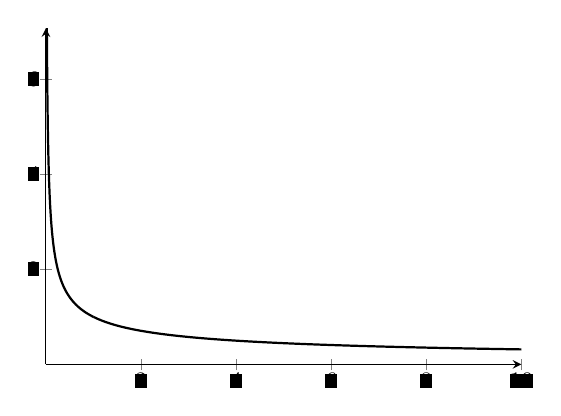
\begin{tikzpicture}
    \begin{axis}[axis equal image, enlarge y limits=false, ymin=0, xmin=0]
      \addplot [domain=.02:1] {1/x^.5}; %
      \addplot [domain=1:10] {1/x^.5}; %
    \end{axis}
  \end{tikzpicture}
  \begin{enumerate}
  \item \label{fall2017-premidterm-2-modified-estimate}
    \begin{problem}[\vfill]
      Use an appropriate secant line to approximate $\dfrac{1}{\sqrt{5}}$. 
    \end{problem}

    \begin{solution}
      We want to approximate $f(5)$, so let's find 2 numbers near 5 where $f$ is easy to evaluate. The closest are 4 and 9, so we'll find the secant line between $(4, f(4))$ and $(9, f(9))$. The slope of this secant line is $\displaystyle \frac{f(9)-f(4)}{9-4}=\frac{\frac{1}{3}-\frac{1}{2}}{5} = - \dfrac{1}{30}$.

      \begin{checkanswer}
        This seems reasonable based on the picture, which shows the secant line should have a negative slope that's close to 0.
      \end{checkanswer}

      Since $\left(4, \frac{1}{2} \right)$ is a point on the secant line, the secant line has equation $\displaystyle y-\frac{1}{2}=-\frac{1}{30}(x-4)$, or $\displaystyle y = -\frac{1}{30}(x-4) + \frac{1}{2}$. Therefore, the height of the secant line when $x = 5$ is $\displaystyle -\frac{1}{30}(5-4) + \frac{1}{2} = \frac{1}{2} - \frac{1}{30} = \boxed{\frac{7}{15}}$.       
    \end{solution}

  \item
    \begin{problem}[\stretch{0.25}]
      Is your answer to \ref{fall2017-premidterm-2-modified-estimate} an overestimate or an underestimate of the actual value of $\dfrac{1}{\sqrt{5}}$? Explain how you know.
    \end{problem}

    \begin{solution}
      The graph of $f$ is concave up, so the secant line between $(4, f(4))$ and $(9, f(9))$ lies above the graph. (At least, the part between $x = 4$ and $x = 9$ does, and that's the part we care about because we plugged in $x = 5$.) So, our estimate is an \fbox{overestimate}. 
    \end{solution}

  \item % added by JC

    \begin{problem}[\nstretch{0.25}]
      Suppose you're interested in the value of $f'(4)$. Write down an expression that you could plug into a calculator to give a reasonable approximation of $f'(4)$. 
    \end{problem}

    \begin{solution}
      We can approximate $f'(4)$ by finding the slope of the secant line between $x = 4$ and $x = \text{a number really close to 4}$. So, for example, we could use the slope of the secant line between $x = 4$ and $x = 4.01$, which is $\dfrac{f(4.01) - f(4)}{4.01 - 4} = \boxed{\dfrac{\dfrac{1}{\sqrt{4.01}} - \dfrac{1}{2}}{0.01}}$. (Of course, you could have used a point other than 4.01.) 
    \end{solution}

  \end{enumerate}

\item  % Fall 2014 Math Ma PS 25, #7
  \points{10}

  The manager of a coffee shop has found that the number of cups of hot chocolate the shop sells each day only depends on the morning temperature outside. Suppose that $C(T)$ is the number of cups of hot chocolate they sell on days when the morning temperature outside is $T$ degrees Fahrenheit.

  \begin{enumerate}

  \item
    \begin{problem}[\stretch{0.25}]
      What are the units of $C'(T)$?
    \end{problem}

    \begin{solution}
      The units are \fbox{number of cups of hot chocolate per $^\circ$F}.  
    \end{solution}

  \end{enumerate}

  Suppose $C'(30) = -10$.

  \begin{enumerate}[resume]

  \item
    \begin{problem}[\vfill]
      Can you reasonably approximate the number of cups of hot chocolate
      sold when the morning temperature is $31^\circ$F?  If so, do it. If
      not, explain why not.
    \end{problem}

    \begin{solution}
      We \fbox{do not have enough information} to do this. All we know about the function $C(T)$ is $C'(30)$, which tells us approximately how a small change in temperature from $30^\circ$F affects the number of cups of hot chocolate sold. However, we don't have any idea how many cups of hot chocolate are sold when the temperature is $30^\circ$F, so we can't approximate the number of cups sold when the temperature is $31^\circ$F. (Graphically, knowing $C'(30)$ tells us the slope of the graph of $C(T)$ at $T = 30$, but we don't know anything about the height of the graph.)
    \end{solution}

  \item
    \begin{problem}[\vfill]
      If the temperature rises from $30^\circ$F one day to $31^\circ$F the next, can you reasonably approximate how many fewer cups of hot chocolate will be sold? If so, do it. If not, explain why not.
    \end{problem}

    \begin{solution}
      Yes, we can do this; knowing that $C'(30) = -10$ means that, when the temperature is $30^\circ$F, the number of cups of hot chocolate sold changes by approximately $-10$ cups per $^\circ$F change in the temperature (for small changes in the temperature). So, when the temperature increases by $1^\circ$F from $30^\circ$, we expect the number of cups of hot chocolate sold to \fbox{decrease by 10}.
    \end{solution}

  \item
    \begin{problem}[\vfill]
      If the temperature drops from $30^\circ$F on October 1 to $28^\circ$F on November 1, can you reasonably approximate how many more cups of hot chocolate will be sold? If so, do it. If not, explain why not.
    \end{problem}

    \begin{solution}
      Yes, we can do this, since it again involves a small change in temperature; a $-2^\circ$F change in temperature should cause a change of roughly ($-10$ cups/$^\circ$F)($-2^\circ$F), which is an \fbox{increase by 20 cups}.
    \end{solution}

  \item
    \begin{problem}[\vfill]
      If the temperature rises from $30^\circ$F one Monday to $55^\circ$F the next Monday, can you reasonably approximate how many fewer cups of hot chocolate will be sold? If so, do it. If not, explain why not.
    \end{problem}

    \begin{solution}
      We can make an approximation, but it's \fbox{not likely to be reasonable}; the derivative is an instantaneous rate of change, so it's only reasonable to use it to look at small changes in temperature. A change from $30^\circ$F to $55^\circ$F is quite large, so we don't expect the derivative to give us a reasonable approximation.
    \end{solution}

  \item

    \begin{problem}[\nstretch{0.25}]
      Let $R(H)$ be the revenue, in dollars, the coffee shop will earn from selling $H$ cups of hot chocolate. Write an expression giving the shop's revenue from selling hot chocolate on a day where the morning temperature outside is $35$ degrees Fahrenheit.
    \end{problem}

    \begin{solution}
      If the morning temperature outside is $35^\circ$F, they will sell $C(35)$ cups of hot chocolate. To get the revenue, we need to plug the number of cups they sell into $R$. So, their revenue is $\boxed{R(C(35))}$. 
    \end{solution}

  \end{enumerate}

\item \label{fall2017-premidterm-4} \points{18}  %KE

  These days, airlines have created complicated pricing schemes for their seats in order to maximize profits by reaching multiple markets.  In this problem, we will consider a simplified model. 

  Suppose Allaboard Airlines has a standard route from Boston to Salt Lake City on a Boeing 737 with 140 seats.  They sell the first 40 seats for \$150 each, the next 40 seats for \$300 each, and the remaining seats for \$400 each.  In this model, assume that all seats are otherwise equivalent, so that customers will always purchase the cheapest seat available.

  \solonly{\related{{{\#4}} on \href{https://people.math.harvard.edu/~jjchen/mathma/docs/worksheets/worksheet05-sols.html}{the worksheet ``Linear and Piecewise Linear Functions''}; \href{https://people.math.harvard.edu/~jjchen/mathma/docs/homework/PS05.html}{Problem Set 5}, {{\#4}}; \href{https://people.math.harvard.edu/~jjchen/mathma/docs/workshops/workshop02.html}{Workshop 2}, {{\#3}}}}

  \begin{enumerate}
  \item \label{fall2017-premidterm-4-graph}
    \begin{problem}
      Let $R(x)$ represent the total revenue from selling $x$ seats. Draw a graph of $R(x)$, labeling any significant points on the graph.
    \end{problem}

    \probonly{\axes[xmin=0, ymin=0, width=4in]}

    \begin{solution}
      From the description, we can tell right away that the graph is piecewise linear with slope $150$ on the interval $(0, 40)$, slope $300$ on $(40, 80)$, and slope $400$ on $(80, 140)$. So, the important points will be when $x = 40$, 80, and 140. Let's find the corresponding revenues:
      \begin{itemize}
      \item The revenue from selling 40 seats is $40 \cdot 150 = 6000$ dollars.

      \item The revenue from selling 80 seats is $40 \cdot 150 + 40 \cdot 300 = 18000$ dollars.

      \item The revenue from selling all 140 seats is $40 \cdot 150 + 40 \cdot 300 + 60 \cdot 400 = 42000$ dollars.
      \end{itemize}
      So, three important points on the graph are $(40, 6000)$, $(80, 18000)$, and $(140, 42000)$.

      \begin{center}
        \answer{
        \begin{tikzpicture}
          \begin{axis}[xtick={40, 80, 140}, ytick={6000, 18000, 42000}, disabledatascaling=false, enlarge x limits=auto]
            \addplot+[sharp plot] coordinates {(0, 0) (40, 6000) (80, 18000) (140, 42000)}; %
            \addplot+[closed] coordinates {(40, 6000) (80, 18000) (140, 42000)}; %
            \addplot+[closed, nodes near coords, point meta=explicit symbolic, node near coords style={anchor=north west}] coordinates {(40, 6000) [(40, 6000)] (80, 18000) [(80, 18000)] (140, 42000) [(140, 42000)]}; %
          \end{axis}
        \end{tikzpicture}
      }
      \end{center}            
    \end{solution}

  \item
    \begin{problem}[\vfill\newpage]
      Write a formula for $R(x)$.
    \end{problem}

    \begin{solution}
      If $x \leq 40$, then $R(x) = 150 x$. If $40 < x \leq 80$, then
      \[ R(x) = \underbrace{150 \cdot 40}_{\text{revenue from first 40 seats}} + \underbrace{300 (x - 40)}_\text{revenue from rest of seats}\] And if $x > 80$, then
      \[ R(x) = \underbrace{150 \cdot 40}_{\text{revenue from first 40 seats}} + \underbrace{300 \cdot 40}_{\text{revenue from next 40 seats}} + \underbrace{400 (x - 80)}_\text{revenue from rest of seats}\]
      So,
      \[ R(x) =
        \boxed{
          \begin{cases}
            150 x & \text{ if } 0 \leq x \leq 40 \\
            300(x-40)+6000 & \text{ if } 40 < x \leq 80 \\
            400(x-80)+18000 & \text{ if } 80 < x \leq 140
          \end{cases}}
      \]
      \begin{checkanswer}
        A good check is to make sure this formula agrees with the important points we labeled on our graph. According to this formula,
        \begin{itemize}[nosep]
        \item $R(40) = 6000$ \check
        \item $R(80) = 300 \cdot 40 + 6000 = 18000$ \check
        \item $R(140) = 400 \cdot 60 + 18000 = 42000$ \check
        \end{itemize}
      \end{checkanswer}
    \end{solution}

  \item
    \begin{problem}[\vfill]
      Allaboard Airlines will break even on this route if they make at least \$20,000 in revenue from the flight. How many seats do they need to sell to break even?
    \end{problem}

    \begin{solution}
      From the graph, we can tell this will happen in the third piece, where $80 < x \leq 140$, so we only need to use that piece of the formula for $R(x)$:
      \begin{align*}
         400(x-80)+18000 &= 20000 \\
         400(x-80)  &= 2000   \\
         x-80  &= 5  \\
         x &= \boxed{85}
       \end{align*}
    \end{solution} 

  \item
    \begin{problem}[\vfill]
      Graph $R'(x)$. Label any significant values on the axes. 
    \end{problem}

    \begin{solution}
      As we said in \ref{fall2017-premidterm-4-graph}, the graph of $R(x)$ has slope $150$ on $(0, 40)$, slope $300$ on $(40, 80)$, and slope $400$ on $(80, 140)$. So, here's the graph of $R'(x)$:
      \begin{center}
        \answer{
          \begin{tikzpicture}
            \begin{axis}[ xtick={40, 80, 140}, ytick={150, 300, 400}, ymin=0, enlarge x limits=auto]
              \addplot[open] coordinates{(0, 150) (140, 400) (40, 150) (40, 300) (80, 300) (80, 400)}; %
              \addplot [domain=0:40] {150}; %
              \addplot [domain=40:80] {300}; %
              \addplot [domain=80:140] {400}; %
            \end{axis}
          \end{tikzpicture}
        }
      \end{center}
    \end{solution}

  \item
    \begin{problem}[\nstretch{0.4}]
      Describe in words what $R'(x)$ represents. Include units.
    \end{problem}

    \begin{solution}
      $R'(x)$ represents the \answer{additional revenue per additional seat sold if the airline has already sold $x$ seats, in dollars per seat}.
    \end{solution}

  \end{enumerate}

\item \label{fall2017-premidterm-6} \points{11} 

  \def\FunctionF(#1){0.1*((#1)^4- 9*(#1)^2)}%
  \def\FunctionG(#1){0.2*((#1)^4- 9*(#1)^2)}%
  \def\FunctionH(#1){0.1*(((#1))^4- 9*((#1))^2)-2}%
  \def\FunctionP(#1){0.1*((2*(#1))^4- 9*(2*(#1))^2)}%
  \def\FunctionQ(#1){0.1*((2*(#1))^4- 9*(2*(#1))^2)-2}%
  \def\FunctionR(#1){-1*(0.1*((#1)^4- 9*(#1)^2))}%

  Here is the graph of $y = f(x)$.

  \begin{tikzpicture}
    \begin{axis}[
      axis y line=center, 
      axis x line=middle, 
      axis on top=false, 
      xmin=-5.5, 
      xmax=5.5, 
      ymin=-5.5, 
      ymax=5.5, 
      height=6cm, 
      width=6cm, 
      grid=both, 
      xtick={-4, -2, 2, 4}, minor xtick={-5, ..., 5},
      ytick={-4, -2, 2, 4}, minor ytick={-5, ..., 5},       
      ]
      \addplot [domain=-5:5] {\FunctionF(x)};
    \end{axis}
  \end{tikzpicture}

  \begin{enumerate} 
  \item
    Each picture below shows $f$ together with the graph of another function (the dashed one); the last graph is identical to $f$. Match each dashed graph with the appropriate function (choices i - viii), and write your answer in the blank below the graph. No explanation is necessary.

    \answeronly{(Going across)}

    \begin{tabular}{ccccc}
      \begin{tikzpicture}
        \begin{axis}[
          axis y line=center, 
          axis x line=middle, 
          axis on top=false, 
          xmin=-5.5, 
          xmax=5.5, 
          ymin=-5.5, 
          ymax=5.5, 
          height=6cm, 
          width=6cm, 
          grid=both, 
          xtick={-4, -2, 2, 4}, minor xtick={-5, ..., 5},
          ytick={-4, -2, 2, 4}, minor ytick={-5, ..., 5},
          ]
          \addplot [domain=-5:5] {\FunctionF(x)};
          \addplot [dashed, domain=-5:5] {\FunctionG(x)};
        \end{axis}
      \end{tikzpicture} 
      &&

      \begin{tikzpicture}
        \begin{axis}[
          axis y line=center, 
          axis x line=middle, 
          axis on top=false, 
          xmin=-5.5, 
          xmax=5.5, 
          ymin=-5.5, 
          ymax=5.5, 
          height=6cm, 
          width=6cm, 
          grid=both, 
          xtick={-4, -2, 2, 4}, minor xtick={-5, ..., 5},
          ytick={-4, -2, 2, 4}, minor ytick={-5, ..., 5},
          ]
          \addplot [domain=-5:5] {\FunctionF(x)};
          \addplot [dashed, domain=-5:5] {\FunctionH(x)};
        \end{axis}
      \end{tikzpicture}
      &&

      \begin{tikzpicture}
        \begin{axis}[
          axis y line=center, 
          axis x line=middle, 
          axis on top=false, 
          xmin=-5.5, 
          xmax=5.5, 
          ymin=-5.5, 
          ymax=5.5, 
          height=6cm, 
          width=6cm, 
          grid=both, 
          xtick={-4, -2, 2, 4}, minor xtick={-5, ..., 5},
          ytick={-4, -2, 2, 4}, minor ytick={-5, ..., 5},
          ]
          \addplot [domain=-5:5] {\FunctionF(x)};
          \addplot [dashed, domain=-3:3] {\FunctionP(x)};
        \end{axis}
      \end{tikzpicture}
      \\
      \cfitb{0.35in}{vii} && \cfitb{0.35in}{i} && \cfitb{0.35in}{iv} \\[24pt]

      \begin{tikzpicture}
        \begin{axis}[
          axis y line=center, 
          axis x line=middle, 
          axis on top=false, 
          xmin=-5.5, 
          xmax=5.5, 
          ymin=-5.5, 
          ymax=5.5, 
          height=6cm, 
          width=6cm, 
          grid=both, 
          xtick={-4, -2, 2, 4}, minor xtick={-5, ..., 5},
          ytick={-4, -2, 2, 4}, minor ytick={-5, ..., 5},
          ]
          \addplot [domain=-5:5] {\FunctionF(x)};
          \addplot [dashed, domain=-5:5] {\FunctionR(x)};
        \end{axis}
      \end{tikzpicture}
      &&

      \begin{tikzpicture}
        \begin{axis}[
          axis y line=center, 
          axis x line=middle, 
          axis on top=false, 
          xmin=-5.5, 
          xmax=5.5, 
          ymin=-5.5, 
          ymax=5.5, 
          height=6cm, 
          width=6cm, 
          grid=both, 
          xtick={-4, -2, 2, 4}, minor xtick={-5, ..., 5},
          ytick={-4, -2, 2, 4}, minor ytick={-5, ..., 5},
          ]
          \addplot [domain=-5:5] {\FunctionF(x)};
          \addplot [dashed, domain=-3:3] {\FunctionQ(x)};
        \end{axis}
      \end{tikzpicture}
      &&
      \begin{tikzpicture}
        \begin{axis}[
          axis y line=center, 
          axis x line=middle, 
          axis on top=false, 
          xmin=-5.5, 
          xmax=5.5, 
          ymin=-5.5, 
          ymax=5.5, 
          height=6cm, 
          width=6cm, 
          grid=both, 
          xtick={-4, -2, 2, 4}, minor xtick={-5, ..., 5},
          ytick={-4, -2, 2, 4}, minor ytick={-5, ..., 5},
          ]
          \addplot [dashed, domain=-5:5] {\FunctionF(x)};
        \end{axis}
      \end{tikzpicture} \\
      \cfitb{0.35in}{vi} && \cfitb{0.35in}{v} && \cfitb{0.35in}{iii}
    \end{tabular} 

    Choices:

    \begin{noanswer}
      \begin{enumeratecols}[label=\roman*.]{4}
      \item $y=f(x)-2$
      \item $y=f\left(\frac{x}{2}\right)$
      \item $y=f(-x)$
      \item $y=f(2x)$
      \item $y=f(2x)-2$
      \item $y=-f(x)$
      \item $y=2f(x)$
      \item $y=2(f(x)-2)$
      \end{enumeratecols}
    \end{noanswer}

    \pspace{\newpage}

  \item % modified slightly by Janet

    In each part, you're given an expression. Pick the choice (A - F) that it represents. You may use each choice A - F once, more than once, or not at all. You might find it helpful to reason on the graph provided, but it isn't actually necessary to answer the question.

    \begin{enumerate}
    \item \cfitb{0.35in}{A} $\displaystyle \frac{f(1) - f(3)}{1-3}$
    \item \cfitb{0.35in}{C} $\displaystyle \lim_{s\to 0}\frac{ f(s) - f(0)}{s}$
    \item \cfitb{0.35in}{D} $\displaystyle \lim_{s\to 0}\frac{f (2+s) - f(2)}{s}$
    \item \cfitb{0.35in}{B} $\displaystyle \lim_{s\to 4}\frac{f(s) - f(1)}{s - 1}$

      \begin{solution}
        The expression $\displaystyle \frac{f(s) - f(1)}{s - 1}$ gives the average rate of change between $x = 1$ and $x = s$. But since $s$ is approaching 4, $\displaystyle \frac{f(s) - f(1)}{s - 1}$ approaches the average rate of change between $x = 1$ and $x = 4$. 
      \end{solution}

    \item \cfitb{0.35in}{A} $\displaystyle \lim_{h \to -2} \frac{f(3 + h) - f(3)}{h}$

      \begin{solution}
        The expression $\displaystyle \frac{f(3 + h) - f(3)}{h}$ gives the average rate of change between $x = 3$ and $x = 3 + h$. Since $h$ is approaching $-2$, the number $3 + h$ is approaching 1, so $\displaystyle \frac{f(3 + h) - f(3)}{h}$ approaches the average rate of change between $x = 3$ and $x = 1$. 
      \end{solution}
    \end{enumerate} 

    Choices:
    \begin{altenumerate}[label=\Alph*.]
    \item average rate of change of $f$ from $x=1$ to $x=3$
    \item average rate of change of $f$ from $x=1$ to $x=4$
    \item instantaneous rate of change of $f$ at $x=0$
    \item instantaneous rate of change of $f$ at $x=2$
    \item instantaneous rate of change of $f$ at $x=3$
    \item none of the above
    \end{altenumerate}

    \pspace{\vfill} 
    \begin{problemonly}
      \begin{center}
        \begin{tikzpicture}[scale=1.]
          \begin{axis}[ axis y line=center, axis x line=middle, axis on top=false, xmin=-5.5, xmax=5.5, ymin=-5.5, ymax=5.5, height=6cm, width=6cm, grid=both, xtick={-4, -2, 2, 4}, minor xtick={-5, ..., 5}, ytick={-4, -2, 2, 4}, minor ytick={-5, ..., 5}, ]
            \addplot [domain=-5:5] {\FunctionF(x)};
          \end{axis}
        \end{tikzpicture}
      \end{center}
    \end{problemonly}
  \end{enumerate}

  \pspace{\newpage} 

\item \label{rectangle-inscribed-in-triangle} \points{12} \finishexam 

  \begin{enumerate}
  \item \label{rectangle-inscribed-in-triangle-function} 
    \begin{problem}[\vfill]
      A right triangle has width 3, height 4, and hypotenuse of length 5. A rectangle is inscribed in the triangle so that its sides are parallel to the legs of the triangle, as shown below. Express the area of the rectangle as a function of its height.

      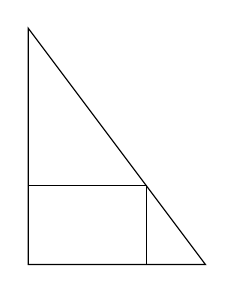
\begin{tikzpicture}[x=0.75cm, y=0.75cm]
        \draw (0, 0) -- (3, 0) -- (0, 4) -- cycle; \draw (0, {4/3}) -- (2, {4/3}) -- (2, 0);
      \end{tikzpicture}
    \end{problem}

    \begin{solution}
      We'll use the same general strategy as in {{\#3}} on \href{https://people.math.harvard.edu/~jjchen/mathma/docs/worksheets/worksheet06-sols.html}{the worksheet ``Function Composition, Modeling with Functions''}: 

      \begin{noanswer}
        \begin{enumerate}[label=\arabic*.]
        \item \hl{\textbf{Understand the Problem.}}

          \begin{itemize}
          \item \hl{\textbf{Goal:}} Express the \goal{area of the rectangle} as a function of its \indvar{height}.

          \item Drawing \textbf{a couple of very different examples} is a great way to get a feel for the situation.
            \begin{center}
              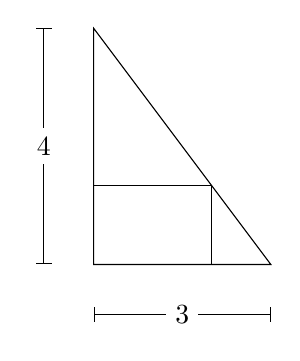
\begin{tikzpicture}[x=0.75cm, y=0.75cm]
                \draw (0, 0) -- (3, 0) -- (0, 4) -- cycle; %
                \draw (0, {4/3}) -- (2, {4/3}) -- (2, 0); \draw[yshift=-18pt, |-|] (0, 0) -- node[fill=white]{3} (3, 0); %
                \draw[xshift=-18pt, |-|] (0, 0) -- node[fill=white]{4} (0, 4); %
              \end{tikzpicture}
              \hspace{0.5in}
              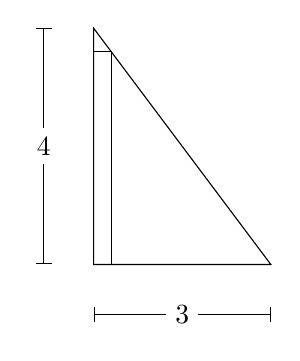
\begin{tikzpicture}[x=0.75cm, y=0.75cm]
                \draw (0, 0) -- (3, 0) -- (0, 4) -- cycle; %
                \draw (0, 3.6) -- (0.3, 3.6) -- (0.3, 0); \draw[yshift=-18pt, |-|] (0, 0) -- node[fill=white]{3} (3, 0); %
                \draw[xshift=-18pt, |-|] (0, 0) -- node[fill=white]{4} (0, 4); %
              \end{tikzpicture}
            \end{center}
          \end{itemize}

        \item Since our goal is the \goal{area of the rectangle}, let's \hl{\textbf{write a formula}} for it, \hl{\textbf{defining any variables we use}}. Here, we'll define variables by labeling them in our picture:

          \begin{center}
            \goal{$A$} = area of rectangle = $xy$

            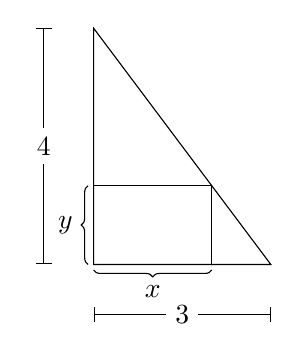
\begin{tikzpicture}[x=0.75cm, y=0.75cm]
              \draw (0, 0) -- (3, 0) -- (0, 4) -- cycle; %
              \draw (0, {4/3}) -- (2, {4/3}) -- (2, 0); %
              \draw[decorate, decoration={brace, mirror}, yshift=-2pt] (0, 0) -- node[below, yshift=-2pt]{$x$} (2, 0); %
              \draw[decorate, decoration={brace}, xshift=-2pt] (0, 0) -- node[left, xshift=-2pt]{$y$} (0, {4/3}); %
              \draw[yshift=-18pt, |-|] (0, 0) -- node[fill=white]{3} (3, 0); %
              \draw[xshift=-18pt, |-|] (0, 0) -- node[fill=white]{4} (0, 4); %
            \end{tikzpicture}
          \end{center}

        \item Now, we need to \hl{\textbf{relate the variables we've used}} ($x$ and $y$) so that we can get everything in terms of the desired variable (\indvar{$y$}). To do this, we must \hl{\textbf{use something else we know about the situation}}. Here, the thing we know is that the rectangle is inscribed in a triangle. From the picture, we can see that the entire triangle is similar to the highlighted triangle:
          \begin{center}
            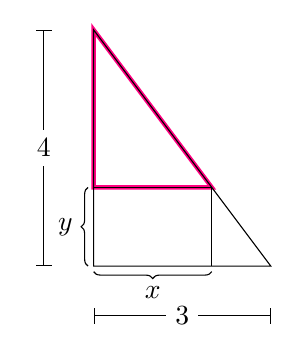
\begin{tikzpicture}[x=0.75cm, y=0.75cm]
              \draw[hotpink, ultra thick] (0, {4/3}) -- (0, 4) -- (2, {4/3}) -- cycle; %
              \draw (0, 0) -- (3, 0) -- (0, 4) -- cycle; %
              \draw (0, {4/3}) -- (2, {4/3}) -- (2, 0); %
              \draw[decorate, decoration={brace, mirror}, yshift=-2pt] (0, 0) -- node[below, yshift=-2pt]{$x$} (2, 0); %
              \draw[decorate, decoration={brace}, xshift=-2pt] (0, 0) -- node[left, xshift=-2pt]{$y$} (0, {4/3}); \draw[yshift=-18pt, |-|] (0, 0) -- node[fill=white]{3} (3, 0); %
              \draw[xshift=-18pt, |-|] (0, 0) -- node[fill=white]{4} (0, 4); %
            \end{tikzpicture}
          \end{center}
          The highlighted triangle has width $x$ and height $4 - y$, so $\dfrac{x}{3} = \dfrac{4 - y}{4}$. Therefore, $x = \dfrac{3 (4 - y)}{4}$; plugging this into our formula for $A$ gives $A$ in terms of just $y$: $ \boxed{A(y) = \frac{3 y (4 - y)}{4}}$.
        \end{enumerate}
      \end{noanswer} \answeronly{$A(y) = \dfrac{3}{4} y (4 - y)$}
    \end{solution}

  \item
    \begin{problem}[\nstretch{0.25}]
      What is the domain of the function in \ref{rectangle-inscribed-in-triangle-function}?
    \end{problem}

    \begin{solution}
      The domain gives the possible values of $y$. In order to get an actual rectangle, we must have $0 < y < 4$, so the domain is $\boxed{(0, 4)}$.
    \end{solution}

  \end{enumerate}

\end{enumerate}

\end{document}
